\section{TPS-ZKPI Design}
\label{sec:design}

\subsection{Overview}

TPS-ZKPI follows a Trusted Proof Service-assisted architecture for policy-private
and auditable consent enforcement. As shown in Figure~\ref{fig:tps-zkpi-workflow},
the workflow binds a provider-committed hidden policy to requester-submitted
authorization evidence through TPS-side proof generation and on-chain proof
verification. The provider registers only a policy commitment on-chain and sends
policy-bound proving material to the TPS off-chain. For each access request,
the TPS constructs the private witness from the hidden policy material and requester
evidence, generates a zero-knowledge proof of policy compliance, and submits
a fixed-format proof statement for ACM verification. The ACM records the
authorization outcome, which is then consumed by the resource access layer.

This design separates confidentiality-sensitive proof generation from public
verification. Policy material and requester evidence remain within the
provider--TPS--requester off-chain boundary, while the blockchain verifies only
a fixed-format proof statement against the provider's policy commitment and session-binding
public inputs. Compared with a requester-prove design in which the requester receives
$P_{enc}$ and the commitment-opening randomness, TPS-ZKPI closes that certain leak to
the requester; the corresponding confidentiality failure now occurs only if the TPS
trust boundary is violated.

\begin{figure*}
    \centering
    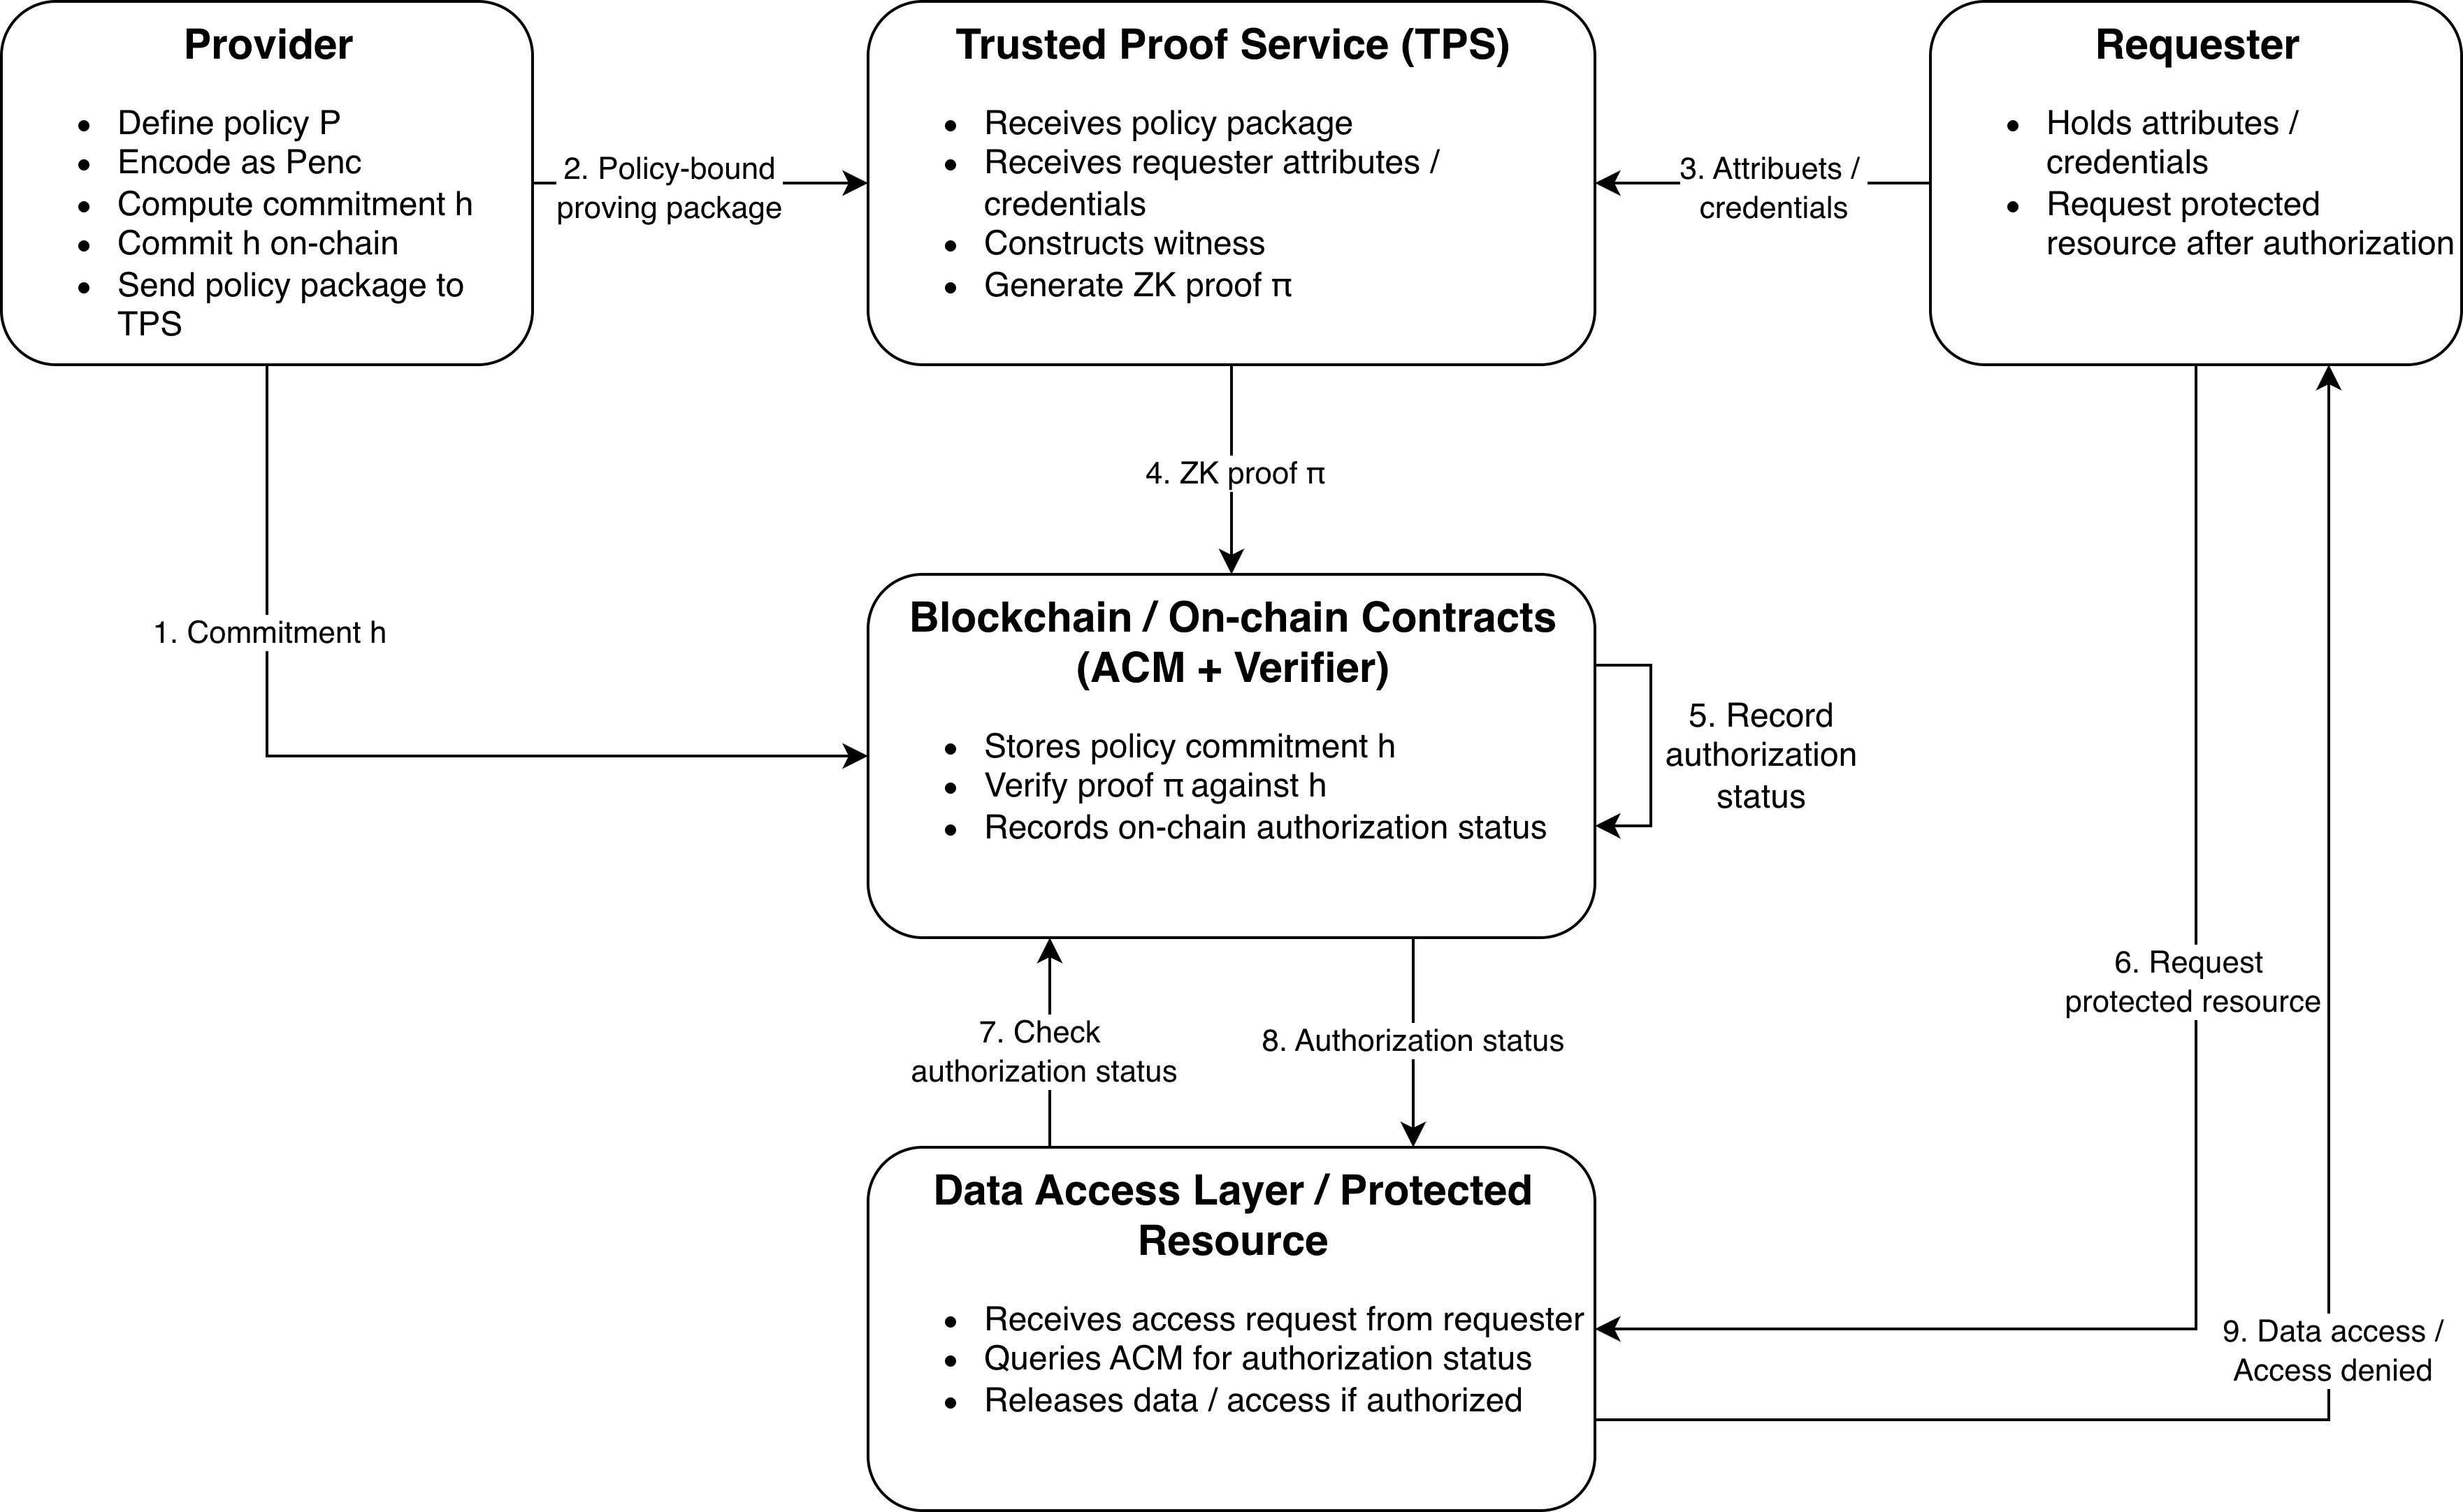
\includegraphics[width=0.6\textwidth]{PP-TPS.png}
    \caption{TPS-assisted policy-compliance workflow.}
    \label{fig:tps-zkpi-workflow}
\end{figure*}

\subsection{Policy Representation and Interpretation}

TPS-ZKPI represents heterogeneous Boolean-based consent policies in a fixed-length,
circuit-friendly format. Let
\begin{equation}
    X = \{0,1\}^{N}, \qquad B = \{0,1\}^{M}
\end{equation}
denote the requester-attribute assignment space and the external-predicate
assignment space, respectively. The full assignment space is
\begin{equation}
    O = X \times B,
\end{equation}
where $a \in X$ encodes requester attributes and $b \in B$ encodes externally
attested predicate outcomes, such as credential validity, ontology-linked checks,
or obligation-related conditions. TPS-ZKPI does not itself solve credential issuance,
revocation, or external attestation; it consumes these outcomes and, where applicable,
checks auxiliary witnesses inside the proof relation. In the current circuit
implementation, issuer-signature verification is represented by a hash-based
placeholder gadget rather than a full EdDSA verifier, so attribute-origin binding is
not enforced in-circuit.

Consent policies are expressed as Boolean formulas over assignment bits:
\begin{equation}
    P ::= atom \mid (P \land P) \mid (P \lor P) \mid \neg P,\qquad
    atom ::= x_i \mid b_j .
\end{equation}
Here $x_i$ selects requester-attribute bit $a_i$ and $b_j$ selects external-predicate
bit $b_j$. Each policy is compiled into a Reverse Polish Notation (RPN) program over
operand tokens, Boolean operator tokens, and deterministic no-op tokens. To support
reusable verification, each program is padded to a fixed token length $L$:
\begin{equation}
    P_{enc}= [t_{1},\ldots,t_{L}],
\end{equation}
where shorter policies are padded with no-op tokens. The implemented circuit uses
$L=\mathsf{DEPTH}=20$; the name \textsf{DEPTH} is an implementation parameter for
RPN token count, not formula nesting depth. No-op tokens are ignored by the stack
semantics and leave the final output unchanged. We denote the set of length-$L$
programs by $\mathsf{Prog}_{L}$.

The reusable policy interpreter is a zero-knowledge circuit
\begin{equation}
    C : \mathsf{Prog}_{L}\times O \rightarrow \{0,1\}.
\end{equation}
Given an encoded policy and operand values, the interpreter evaluates the
RPN program using deterministic stack semantics and enforces well-formedness
constraints inside the circuit. The circuit outputs $1$ only if the program is
syntactically valid and the requester evidence satisfies the encoded policy.
An output of $0$ is not diagnostic: it may mean either a malformed program or
unsatisfied evidence. The proved acceptance relation is therefore the asserted
case $C(P_{enc},(a,b))=1$.
This interpreter is a fixed-operand stack-based RPN evaluator, not a general policy
language runtime.

This design avoids policy-specific circuits and verifier contracts while supporting
policy evolution through different fixed-length policy programs.

\subsection{Commitment Binding and Proof Generation}

To bind each proof to a provider-defined hidden policy, the provider samples
commitment randomness $r$ uniformly from the scalar field and computes
\begin{equation}
    h = \mathsf{Com}(P_{enc}; r) = \mathsf{Poseidon}(P_{enc}\parallel r),
\end{equation}
where $h$ is stored on-chain as the public handle of the hidden policy. The
commitment binds future proofs to the committed policy instance under the
collision resistance of Poseidon. Hiding is an explicit commitment assumption that
relies on high-entropy $r$ and the fixed-length encoding of $P_{enc}$, which keeps the
sponge input unambiguous.

For an access request, the TPS constructs the private witness
\begin{equation}
    w = (P_{enc}, a, b, r, \omega),
\end{equation}
where $P_{enc}$ is the encoded policy, $a$ denotes requester attributes, $b$
denotes external predicate outcomes, $r$ is the commitment randomness, and $\omega$
denotes auxiliary witnesses for credential- or predicate-dependent checks. The
public statement contains the policy commitment $h$, requester and resource
identifiers, a session nonce, and fixed-format public parameters $pp$.

For the compiled circuit and Groth16 common reference string, setup produces a proving
key and verification key:
\begin{equation}
    (pk, vk) \leftarrow \mathsf{Setup}(C).
\end{equation}
The TPS generates a proof
\begin{equation}
    \pi \leftarrow \mathsf{Prove}\bigl(pk, w; (h, id_{req}, id_{res}, nonce, pp)\bigr).
\end{equation}
The proof certifies the conjunction that
$C(P_{enc},(a,b))=1$, the hidden policy encoding is consistent with the on-chain
commitment $h$, required external-predicate checks are internally consistent with
respect to the supplied parameters and placeholder gadgets, and the proof is bound to
the requester, resource, and session context.

The ACM verifies $\pi$ on-chain against $vk$ and the public statement. If
verification succeeds, it records a positive authorization outcome for the requester
and resource. The policy encoding, commitment randomness, requester
attributes, credential witnesses, and auxiliary proof material are not
posted on-chain.

\subsection{Transcript Normalization}

Zero-knowledge proofs hide private witness values, but surrounding
blockchain artifacts may still leak policy-dependent information. TPS-ZKPI therefore
normalizes the public transcript so that different policies induce fixed or tightly
bounded observable profiles. Table~\ref{tab:transcript-normalization}
summarizes the mechanisms.

\begin{table}[ht]
    \centering
    \caption{Transcript-normalization mechanisms in TPS-ZKPI.}
    \label{tab:transcript-normalization} \footnotesize
    \begin{tabular}{p{0.24\linewidth}p{0.66\linewidth}}
        \hline
        \textbf{Artifact} & \textbf{Normalization mechanism}                                          \\
        \hline
        Calldata          & Fixed verification interface and padded proof/public-input encoding.      \\
        Logs              & Fixed event structure with constant topic and payload layout.             \\
        Public parameters & Fixed-format handles instead of policy artifacts or credential witnesses. \\
        Gas usage         & Policy-independent verifier logic with bounded or padded gas profiles.    \\
        \hline
    \end{tabular}
\end{table}

These mechanisms do not eliminate all public observability. Rather, they reduce
policy-dependent variation in calldata, logs, public parameters, and gas-related
behavior that could otherwise serve as a fingerprint for the metadata-only
adversary defined in Section~\ref{sec:problem}. TPS-ZKPI does not flatten all
residual channels: timing between transactions, transaction ordering, mempool or
broadcast patterns, and off-chain TPS communication remain outside the normalized
public transcript.
